\documentclass[a4paper, 12pt]{article}

\usepackage{graphicx}
\graphicspath{{./images/}}
\usepackage{float}
\usepackage{wrapfig}
\usepackage{blindtext}
\usepackage{amsmath}
\usepackage{amssymb}
\usepackage{fancyhdr}
\usepackage[margin=0.9in]{geometry}
\usepackage[sorting = none]{biblatex}
\addbibresource{progress.bib}
\usepackage[colorlinks=true,linkcolor=red, citecolor=black, urlcolor = black]{hyperref}%
\usepackage{appendix}
\usepackage{pythonhighlight}
\usepackage{subcaption}

\begin{document}

\title{\textbf{GW Burst Progress Documentation}}
\author{Ethan Millar}
\date{}
\maketitle

\section{Adding Noise}
\subsection{Troubleshooting}

\begin{figure}[H]
  \centering
  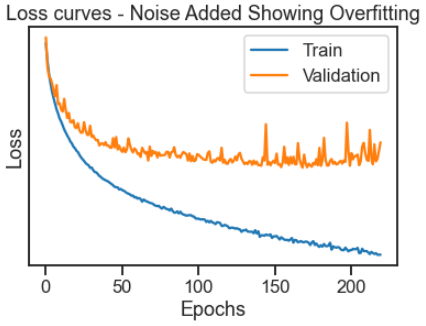
\includegraphics[scale = 0.5]{Overfit.PNG}
  \caption{Loss curves comparing training and validation set demonstrating overfitting in the model}
  \label{fig:overfit}
\end{figure}

Steps relating to the model were taken to try and optimise the model, first attempt was with regularisation, in particular altering the weight decay parameter in the adam optimiser from $1 \times 10^{-6}$ to $  \times 10^{-4}$.

I ran the first 50 epochs to compare to the initial overfitted curves

\begin{figure}[H]
\begin{subfigure}{.5\textwidth}
    \centering
    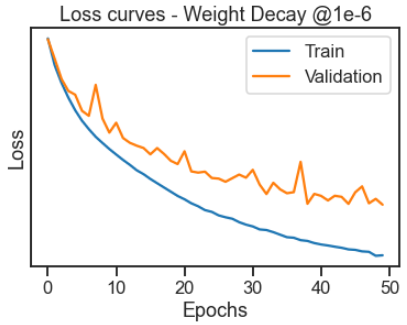
\includegraphics[width=1\textwidth, scale = 0.1]{Weightdecay0.PNG}
    \caption{Loss curves after increasing the weight decay to $1 \times 10^{-6}$}
    \label{fig:wd0}
\end{subfigure} \hfill
\begin{subfigure}{.4\textwidth}
    \centering
    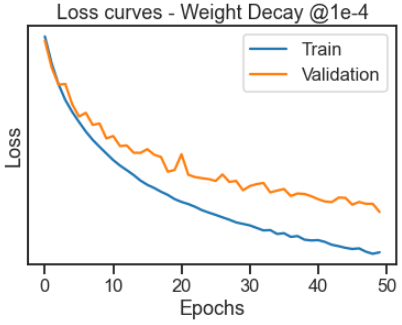
\includegraphics[width=1.1\textwidth, scale = 0.2]{Weightdecay1.PNG}
    \caption{Loss curves after increasing the weight decay to $1 \times 10^{-4}$}
    \label{fig:wd1}
\end{subfigure} \hfill
\begin{subfigure}{.4\textwidth}
    \centering
    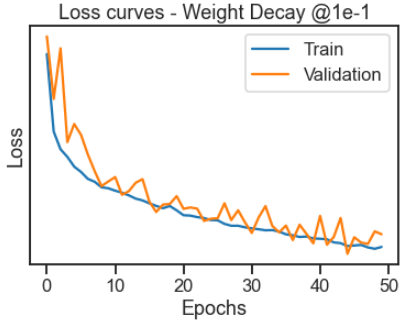
\includegraphics[width=1.1\textwidth, scale = 0.2]{Weightdecay2.PNG}
    \caption{Loss curves after increasing the weight decay to $1 \times 10^{-1}$}
    \label{fig:wd2}
\end{subfigure}%
\centering
\caption{Comparing Loss Curves when altering weight decay}

\end{figure}

\begin{figure}[H]
  \centering
  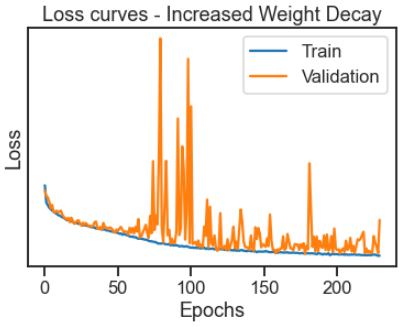
\includegraphics[scale = 0.5]{LossSpikes.PNG}
  \caption{Running for 225 epochs with the weight decay increased to $1 \times 10^{-1}$}
  \label{}
\end{figure}

Next approach is to decrease the learning rate from $1 \times 10^{-3}$ to $1 \times 10^{-4}$

Having altered the flow this is what was being produced:

\begin{figure}[H]
\begin{subfigure}{.5\textwidth}
    \centering
    \includegraphics[width=1\textwidth, scale = 0.5]{loss0.PNG}
    \caption{Loss curves after altering the weight decay to $1 \times 10^{-1}$ and the learning rate to $1 \times 10^{-4}$}
    \label{fig:lc1}
\end{subfigure} \hfill
\begin{subfigure}{.4\textwidth}
    \centering
    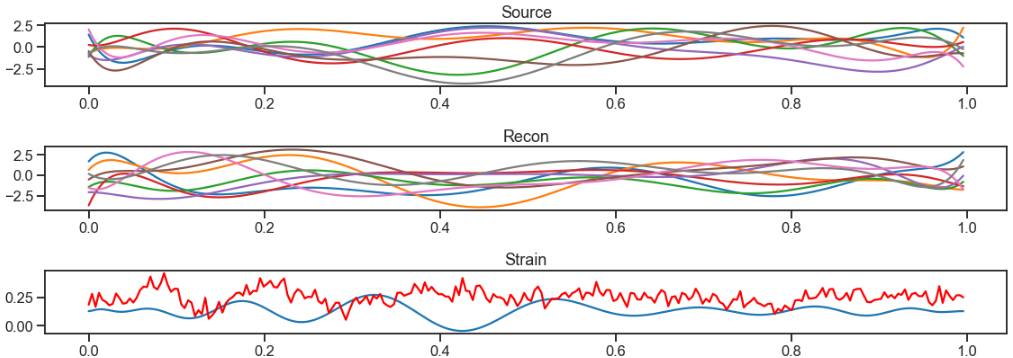
\includegraphics[width=1.1\textwidth, scale = 0.5]{recon1.PNG}
    \caption{Single sample example of the reconstructed mass dynamics and corresponding strain with 1 mass showing 1 reconstruction}
    \label{fig:massrec1}
\end{subfigure} \hfill
\begin{subfigure}{.4\textwidth}
    \centering
    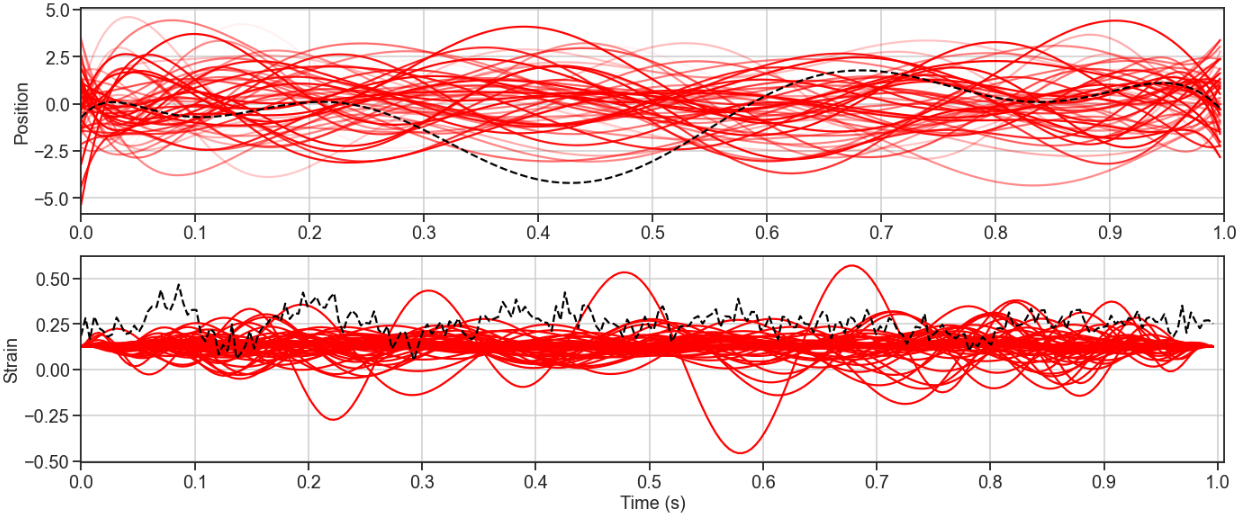
\includegraphics[width=1.1\textwidth, scale = 0.5]{recon50.PNG}
    \caption{Single sample example of the reconstructed mass dynamics and corresponding strain with 1 mass showing 50 reconstructions.}
    \label{fig:massrec01}
\end{subfigure}%
\centering
\caption{Demonstrating loss curves and corresponding test plots with a bug in the code}

\end{figure}

Overall this looked very strange, the loss curves were more closely correlated, but they were very oddly shaped. This was confirmed when plotting the constructed dynamics and strains which shows an offset in the y axis. This was remedied by fixing a bug, afterward I was able to revert back to the original settings of the flow (learning rate of $1 \times 10^{-3}$ and weight decay of $1 \times 10^{-6}$) with the following plots:

\begin{figure}[H]
\begin{subfigure}{.5\textwidth}
    \centering
    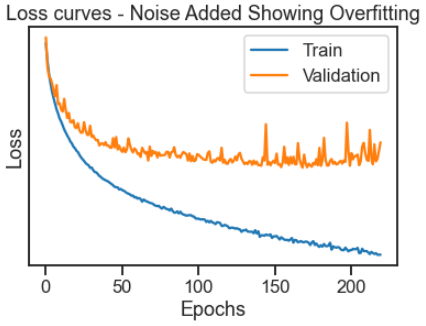
\includegraphics[width=1\textwidth, scale = 0.5]{Overfit.PNG}
    \caption{Loss curves after altering the weight decay to $1 \times 10^{-1}$ and the learning rate to $1 \times 10^{-4}$}
    \label{fig:lc2}
\end{subfigure} \hfill
\begin{subfigure}{.4\textwidth}
    \centering
    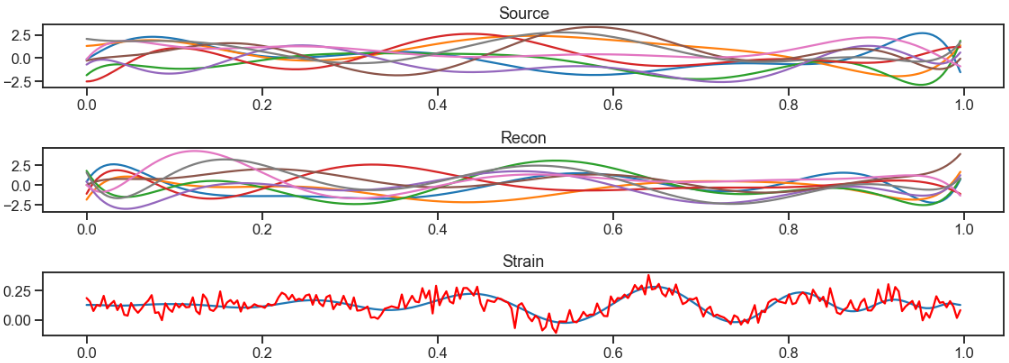
\includegraphics[width=1.1\textwidth, scale = 0.5]{rec1center.PNG}
    \caption{Single sample example of the reconstructed mass dynamics and corresponding strain with 1 mass showing 1 reconstruction}
    \label{fig:massreccenter}
\end{subfigure} \hfill
\begin{subfigure}{.4\textwidth}
    \centering
    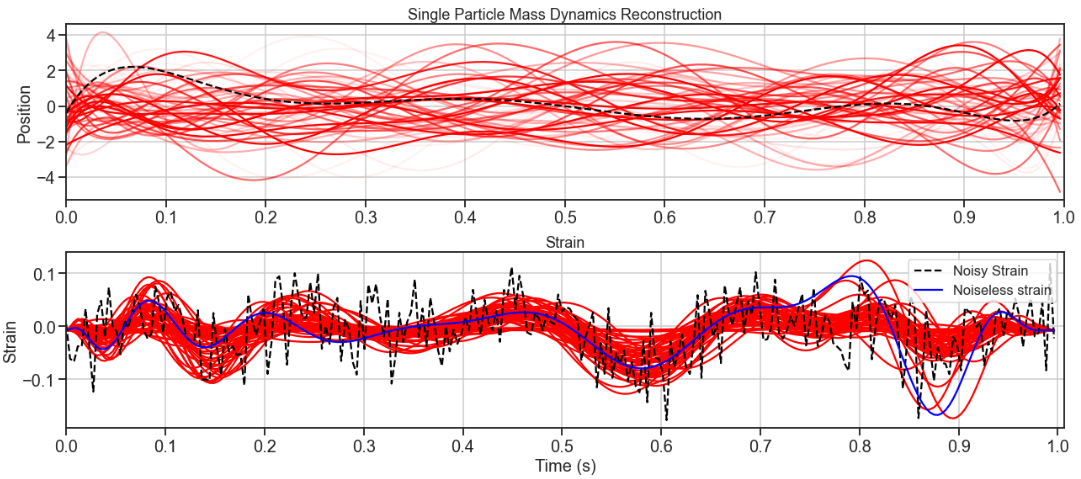
\includegraphics[width=1.1\textwidth, scale = 0.5]{superimpstrains.PNG}
    \caption{Single sample example of the reconstructed mass dynamics and corresponding strain with 1 mass showing 50 reconstructions.}
    \label{fig:massrec50center}
\end{subfigure}%
\centering
\caption{Demonstrating loss curves and corresponding test plots after bug fixing}

\end{figure}

We are able to get reasonable results despite the overfitting as when the data is trained we are using the version which produces the lowest loss in the training data, so despite the overfitting the model is still useable to test.

The next steps from here to optimise the flow in order to reduce or completely eliminate overfitting.

\subsection{Optimising the Flow}

The easiest first step to take is to increase the size of the training data set, with quadrupling the data size we get much closer to fixing the overfitting issue:

\begin{figure}[H]
  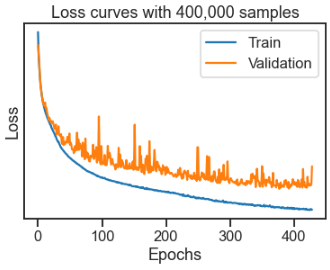
\includegraphics[scale = 0.8]{loss400k}
  \caption{}
  \label{}
\end{figure}

However if we were to go any further we would start to become very computationally costly as this took 5 hours to train, so we look closer at the parameters of the flow.

\section{Going to Higher Dimensions}



\end{document}
